% GNUPLOT: LaTeX picture with Postscript
\begingroup
  \makeatletter
  \providecommand\color[2][]{%
    \GenericError{(gnuplot) \space\space\space\@spaces}{%
      Package color not loaded in conjunction with
      terminal option `colourtext'%
    }{See the gnuplot documentation for explanation.%
    }{Either use 'blacktext' in gnuplot or load the package
      color.sty in LaTeX.}%
    \renewcommand\color[2][]{}%
  }%
  \providecommand\includegraphics[2][]{%
    \GenericError{(gnuplot) \space\space\space\@spaces}{%
      Package graphicx or graphics not loaded%
    }{See the gnuplot documentation for explanation.%
    }{The gnuplot epslatex terminal needs graphicx.sty or graphics.sty.}%
    \renewcommand\includegraphics[2][]{}%
  }%
  \providecommand\rotatebox[2]{#2}%
  \@ifundefined{ifGPcolor}{%
    \newif\ifGPcolor
    \GPcolortrue
  }{}%
  \@ifundefined{ifGPblacktext}{%
    \newif\ifGPblacktext
    \GPblacktexttrue
  }{}%
  % define a \g@addto@macro without @ in the name:
  \let\gplgaddtomacro\g@addto@macro
  % define empty templates for all commands taking text:
  \gdef\gplbacktext{}%
  \gdef\gplfronttext{}%
  \makeatother
  \ifGPblacktext
    % no textcolor at all
    \def\colorrgb#1{}%
    \def\colorgray#1{}%
  \else
    % gray or color?
    \ifGPcolor
      \def\colorrgb#1{\color[rgb]{#1}}%
      \def\colorgray#1{\color[gray]{#1}}%
      \expandafter\def\csname LTw\endcsname{\color{white}}%
      \expandafter\def\csname LTb\endcsname{\color{black}}%
      \expandafter\def\csname LTa\endcsname{\color{black}}%
      \expandafter\def\csname LT0\endcsname{\color[rgb]{1,0,0}}%
      \expandafter\def\csname LT1\endcsname{\color[rgb]{0,1,0}}%
      \expandafter\def\csname LT2\endcsname{\color[rgb]{0,0,1}}%
      \expandafter\def\csname LT3\endcsname{\color[rgb]{1,0,1}}%
      \expandafter\def\csname LT4\endcsname{\color[rgb]{0,1,1}}%
      \expandafter\def\csname LT5\endcsname{\color[rgb]{1,1,0}}%
      \expandafter\def\csname LT6\endcsname{\color[rgb]{0,0,0}}%
      \expandafter\def\csname LT7\endcsname{\color[rgb]{1,0.3,0}}%
      \expandafter\def\csname LT8\endcsname{\color[rgb]{0.5,0.5,0.5}}%
    \else
      % gray
      \def\colorrgb#1{\color{black}}%
      \def\colorgray#1{\color[gray]{#1}}%
      \expandafter\def\csname LTw\endcsname{\color{white}}%
      \expandafter\def\csname LTb\endcsname{\color{black}}%
      \expandafter\def\csname LTa\endcsname{\color{black}}%
      \expandafter\def\csname LT0\endcsname{\color{black}}%
      \expandafter\def\csname LT1\endcsname{\color{black}}%
      \expandafter\def\csname LT2\endcsname{\color{black}}%
      \expandafter\def\csname LT3\endcsname{\color{black}}%
      \expandafter\def\csname LT4\endcsname{\color{black}}%
      \expandafter\def\csname LT5\endcsname{\color{black}}%
      \expandafter\def\csname LT6\endcsname{\color{black}}%
      \expandafter\def\csname LT7\endcsname{\color{black}}%
      \expandafter\def\csname LT8\endcsname{\color{black}}%
    \fi
  \fi
    \setlength{\unitlength}{0.0500bp}%
    \ifx\gptboxheight\undefined%
      \newlength{\gptboxheight}%
      \newlength{\gptboxwidth}%
      \newsavebox{\gptboxtext}%
    \fi%
    \setlength{\fboxrule}{0.5pt}%
    \setlength{\fboxsep}{1pt}%
\begin{picture}(8640.00,8640.00)%
    \gplgaddtomacro\gplbacktext{%
      \csname LTb\endcsname%
      \put(762,4488){\makebox(0,0)[r]{\strut{}$-12$}}%
      \csname LTb\endcsname%
      \put(762,5160){\makebox(0,0)[r]{\strut{}$-8$}}%
      \csname LTb\endcsname%
      \put(762,5832){\makebox(0,0)[r]{\strut{}$-4$}}%
      \csname LTb\endcsname%
      \put(762,6503){\makebox(0,0)[r]{\strut{}$0$}}%
      \csname LTb\endcsname%
      \put(762,7175){\makebox(0,0)[r]{\strut{}$4$}}%
      \csname LTb\endcsname%
      \put(3101,5711){\makebox(0,0)[l]{\strut{}R=0.2}}%
      \csname LTb\endcsname%
      \put(2255,5015){\makebox(0,0)[l]{\strut{}PbPb-pp, 0-30\%}}%
    }%
    \gplgaddtomacro\gplfronttext{%
      \csname LTb\endcsname%
      \put(261,5831){\rotatebox{-270}{\makebox(0,0){\strut{}$\langle \slashed{p}_T^{\parallel} \rangle$}}}%
    }%
    \gplgaddtomacro\gplbacktext{%
      \csname LTb\endcsname%
      \put(6125,5711){\makebox(0,0)[l]{\strut{}R=0.3}}%
    }%
    \gplgaddtomacro\gplfronttext{%
    }%
    \gplgaddtomacro\gplbacktext{%
      \csname LTb\endcsname%
      \put(762,1464){\makebox(0,0)[r]{\strut{}$-12$}}%
      \csname LTb\endcsname%
      \put(762,2136){\makebox(0,0)[r]{\strut{}$-8$}}%
      \csname LTb\endcsname%
      \put(762,2808){\makebox(0,0)[r]{\strut{}$-4$}}%
      \csname LTb\endcsname%
      \put(762,3479){\makebox(0,0)[r]{\strut{}$0$}}%
      \csname LTb\endcsname%
      \put(762,4151){\makebox(0,0)[r]{\strut{}$4$}}%
      \csname LTb\endcsname%
      \put(1139,1110){\makebox(0,0){\strut{}0.1}}%
      \csname LTb\endcsname%
      \put(1414,1110){\makebox(0,0){\strut{}}}%
      \csname LTb\endcsname%
      \put(1688,1110){\makebox(0,0){\strut{}0.5}}%
      \csname LTb\endcsname%
      \put(1963,1110){\makebox(0,0){\strut{}}}%
      \csname LTb\endcsname%
      \put(2238,1110){\makebox(0,0){\strut{}0.9}}%
      \csname LTb\endcsname%
      \put(2513,1110){\makebox(0,0){\strut{}}}%
      \csname LTb\endcsname%
      \put(2788,1110){\makebox(0,0){\strut{}1.3}}%
      \csname LTb\endcsname%
      \put(3063,1110){\makebox(0,0){\strut{}}}%
      \csname LTb\endcsname%
      \put(3337,1110){\makebox(0,0){\strut{}1.7}}%
      \csname LTb\endcsname%
      \put(3612,1110){\makebox(0,0){\strut{}}}%
      \csname LTb\endcsname%
      \put(3101,2687){\makebox(0,0)[l]{\strut{}R=0.4}}%
    }%
    \gplgaddtomacro\gplfronttext{%
      \csname LTb\endcsname%
      \put(261,2807){\rotatebox{-270}{\makebox(0,0){\strut{}$\langle \slashed{p}_T^{\parallel} \rangle$}}}%
      \csname LTb\endcsname%
      \put(2375,831){\makebox(0,0){\strut{}$\Delta$}}%
    }%
    \gplgaddtomacro\gplbacktext{%
      \csname LTb\endcsname%
      \put(4163,1110){\makebox(0,0){\strut{}0.1}}%
      \csname LTb\endcsname%
      \put(4438,1110){\makebox(0,0){\strut{}}}%
      \csname LTb\endcsname%
      \put(4712,1110){\makebox(0,0){\strut{}0.5}}%
      \csname LTb\endcsname%
      \put(4987,1110){\makebox(0,0){\strut{}}}%
      \csname LTb\endcsname%
      \put(5262,1110){\makebox(0,0){\strut{}0.9}}%
      \csname LTb\endcsname%
      \put(5537,1110){\makebox(0,0){\strut{}}}%
      \csname LTb\endcsname%
      \put(5812,1110){\makebox(0,0){\strut{}1.3}}%
      \csname LTb\endcsname%
      \put(6087,1110){\makebox(0,0){\strut{}}}%
      \csname LTb\endcsname%
      \put(6361,1110){\makebox(0,0){\strut{}1.7}}%
      \csname LTb\endcsname%
      \put(6636,1110){\makebox(0,0){\strut{}}}%
      \csname LTb\endcsname%
      \put(6125,2687){\makebox(0,0)[l]{\strut{}R=0.5}}%
    }%
    \gplgaddtomacro\gplfronttext{%
      \csname LTb\endcsname%
      \put(5399,831){\makebox(0,0){\strut{}$\Delta$}}%
      \csname LTb\endcsname%
      \put(6123,2393){\makebox(0,0)[r]{\strut{}8.0-300.0}}%
      \csname LTb\endcsname%
      \put(6123,2207){\makebox(0,0)[r]{\strut{}4.0-8.0}}%
      \csname LTb\endcsname%
      \put(6123,2021){\makebox(0,0)[r]{\strut{}2.0-4.0}}%
      \csname LTb\endcsname%
      \put(6123,1835){\makebox(0,0)[r]{\strut{}1.0-2.0}}%
      \csname LTb\endcsname%
      \put(6123,1649){\makebox(0,0)[r]{\strut{}0.5-1.0}}%
      \csname LTb\endcsname%
      \put(6123,1463){\makebox(0,0)[r]{\strut{}$\langle \slashed{p}_T^{\parallel} \rangle_{\Delta}$}}%
    }%
    \gplbacktext
    \put(0,0){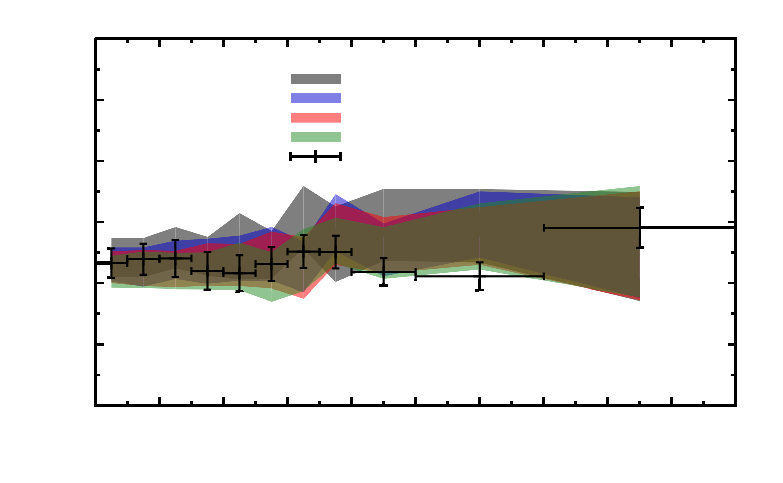
\includegraphics{raa}}%
    \gplfronttext
  \end{picture}%
\endgroup
